\subsection{Background and History}
3D animation can be a painstakingly tedious activity. To create a desired animation, animators go through the long process of key framing. Key frames are set positions that define the start and end points of a movement, sequences of poses in time. Typically, animators assign poses to certain frames over time, so that in-between motions can be generated by a computer. To get an accurate animation, artists usually must assign many key frames, then spend time adjusting and editing them to be more precise. The fact that industry professionals take so much time and effort to do this shows that for an amateur or untrained artist, creating good 3D animation is close to impossible.

\begin{figure}[H]
\centering
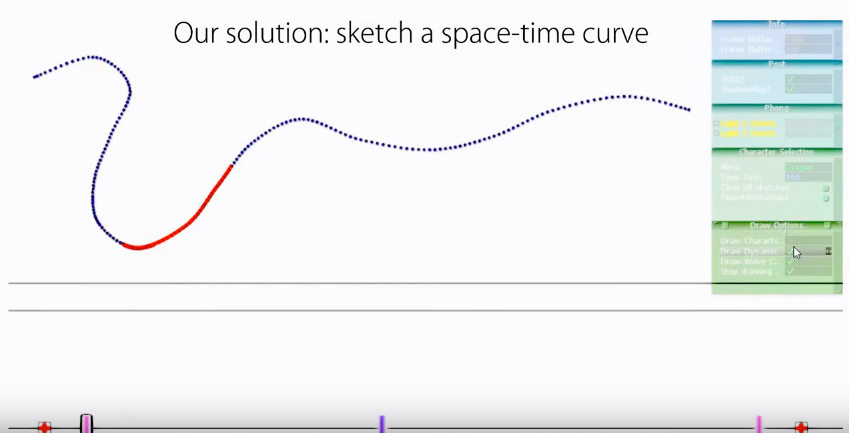
\includegraphics[scale=0.25]{spacetimecurve}
\caption{Drawing of INRIA's space-time curve}
\label{fig:spaceTimeCurve}
\end{figure}

Researchers in the IMAGINE group at INRIA (in Grenoble, France) have noticed this problem \cite{hal}. They have made significant progress on a project called ERC Expressive, where they aim to offer more intuitive tools to author 3D digital content. The IMAGINE team has invented a technique for animation called space-time sketching, in which a user can draw a line in the path they want a model to take and it will be animated accordingly. As the character follows the path, its model bends and changes shape in a physically realistic way. Their system currently supports creating different movements with the path such as bouncing, rolling, and twisting.

\begin{figure}[!htb]
\minipage{0.32\textwidth}
  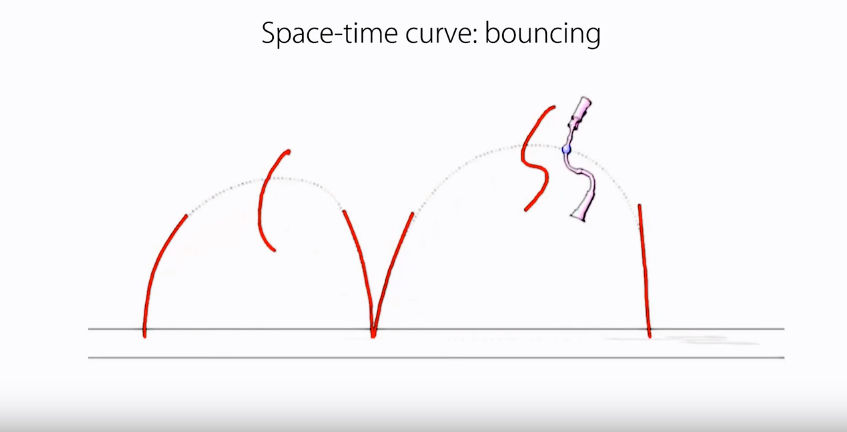
\includegraphics[width=\linewidth]{bouncing}
  \caption{Bouncing}\label{fig:bouncing}
\endminipage\hfill
\minipage{0.32\textwidth}
  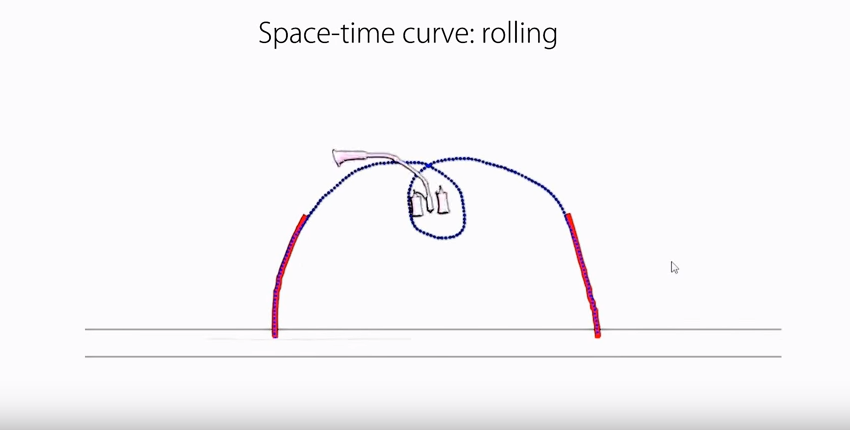
\includegraphics[width=\linewidth]{rolling}
  \caption{Rolling}\label{fig:rolling}
\endminipage\hfill
\minipage{0.32\textwidth}%
  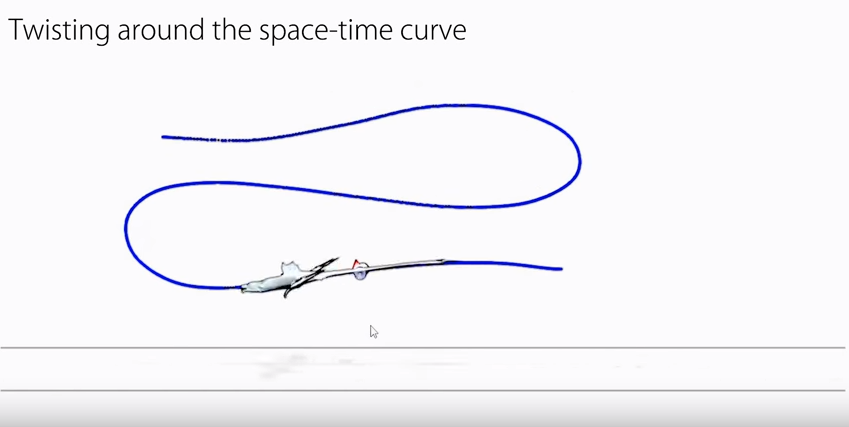
\includegraphics[width=\linewidth]{twisting}
  \caption{Twisting}\label{fig:twisting}
\endminipage
\end{figure}

Because IMAGINE's tool is a comprehensive system that has not yet been released, we want to develop a smaller version of this functionality within a plug-in for the game engine, Unity. One of the main goals of the IMAGINE team's research is to make animation more accessible to the general public. We share this goal, and want to narrow it down specifically to game developers. Many game developers (both amateur and professional) use Unity to make successful games, but some lack the artistic training to integrate high quality animations easily. Our plug-in aims to alleviate this task using INRIA's space-time sketching technique. 

We also want to allow for an animator to specify exceptions to the motions calculated by the algorithm so we will implement a variant of INRIA's technique. Our system will incorporate the notion of the ``default animation" for a shape, and be able to handle exceptions to it. For example, if a user wants to edit a motion they've made for a character, they will be able to specify a point on the drawn path where the motion will vary. To develop such an exception, we will take the original algorithm, recast it in  terms of constraint satisfaction in a non-monotonic language, and add enough apparatus to specify exceptions and deal with them.
